%%\documentclass[a4paper,12pt,twoside]{report}
\documentclass[a4paper,10pt]{report}

%% Je suis englishophone !
\usepackage[english]{babel}
\usepackage[T1]{fontenc}
\usepackage{palatino}
\usepackage{float} %%force a mettre mon image ou je veux
\usepackage{color}

%% Je veux pouvoir inclure des figures...
%% a commenter si vous voulez faire du DVI :
%\usepackage{epstopdf}
\usepackage[pdftex]{graphicx}

%% ... des figures ``jpeg'' ou ``pdf''
%% a commenter si vous voulez faire du DVI :
\DeclareGraphicsExtensions{.jpg,.pdf}

%% Je veux creer des Hyperdocuments
%% a commenter si vous voulez faire du DVI :
%
\usepackage[colorlinks=true,linkcolor=blue,urlcolor=blue]{hyperref}

\usepackage{amssymb}

%%%%%%%%%%%%%%%%%%%%%%%%%%%%%%%%%%%%%%
%% pour citer une figure :
\newcommand{\figref}[1]{figure~\ref{#1}}

%% pour citer une equation :
\newcommand{\Ref}[1]{(\ref{#1})}

%%Set les couleurs
\definecolor{blue}{rgb}{0.2,0.45,0.9}

%% pour mettre l'emphase sur un mot ou un groupe de mots :
\newcommand{\empha}[1]{\textbf{\color{blue}{#1}}}


\title{Techniques de Developpement}
\author{Chaillou Damien \\ Schiaucu Alexandru}
\date{2010}

%Corps du document :
\begin{document}

	\maketitle
	\tableofcontents


	\chapter*{Preface}

		\section{Audience}
			
			This document addresses to two categories of people, according to their needs:
			\begin{itemize}
				\item Players\\
					We created this game mainly for the final player. Everyone interested in the \empha{Go} game could find in the first chapter of this report, named  \textsl{Presentation of the project}\ the light first rules of this game. Then players will be interested to read chapter \textsl{How to play}\, which helps the user to adapt with our application.

				\item Developers\\
					Developers have the possibility to extend or improve our implementation. It is necessary to read chapter \textsl{Presentation of the project}, in order to understand firstly the background and secondly the game itself. Then the \textsl{Software's architecture} chapter will concern the developer only. In this chapter he can read, respectively, the technics and heuristics used, the architecture and then the implementation.
			\end{itemize}		
			
		\section{Organization of This Book}
			This book is organized as the following:
			\begin{itemize}
				\item \textbf{Chapter 1}: \textsl{Presentation of the game}\\ 
					This chapter does a presentation of the \empha{Go} game.
				\item \textbf{Chapter 2}: \textsl{How to play}\\
					In this chapter, we will present to the user how to install the game. Then we will see how to play.

				\item \textbf{Chapter 3}: \textsl{Software's architecture}\\
					Finally we will study the core of the application. We will first describe the algorithms and the heuristics used. Then we will take a look at the architecture, to finally end with the implementation in the Java language.
 

			\end{itemize}		
			
						


	\chapter*{Game presentation}
		\section{Go game - Explanations}
	The Atari-Go game is a simpler version of Go. Go is a millenar game, appeared in China and played in Japon for more than 1200 years. A board (named \empha{Goban}) is a grid of 9 x 9 (in our implementation of the Atari-Go). Each player playes stones of \empha{White} and \empha{Black} colours. The stones must be put on the intersections of this grid.
\
The goal of the game is to capture the opponent's stones, framing one of his groups of stones, thus not leaving him any liberty. The first who takes a group of stones wins the game.
\
This game represents one of the last for which there are no computer programs to match the best human players. Consequently, it is a challenge in Artificial Intelligence. The complexity of Go comes from the difficulty to evaluate a situation on the board and also from the huge branching factor in tree research.



	\chapter*{How to play}
		\section{Running}
			This project has been set up with Maven. There is nothing more simple than generating a Jar executable in order to run the game. The maven command is then:
			\\
			\empha{mvn package}
			\\
			The jar named almago-1.0-SNAPSHOT.jar will be created in the \empha{target} folder. And you can easily run it with the following command:
			\\
			\empha{java -jar almago-1.0-SNAPSHOT.jar}

		\section{Stone selection}
			The user (named "Human" in the GUI) selects the colour of the stones with which he would like to play; this depends on whether he chooses to be the one who starts the game or not. He can do this selection in the two combo-boxes especially created.
The user has the possibility to play White Stone (combo-box \empha{White Stone}), in which case he starts, or Black Stone (combo-box \empha{Black Stones})
			\\
			\begin{center}
				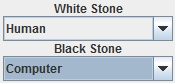
\includegraphics[width=0.30\textwidth] {img/StoneSelect.jpg}
			\end{center}
			
		\section{Difficulty level selection}
		The difficulty level varies between four choices: \empha{Very Easy}, \empha{Easy}, \empha{Medium} and \empha{Hard}
			\\
			\begin{center}
				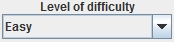
\includegraphics[width=0.30\textwidth] {img/DifficultySelect.jpg}
			\end{center}

		\section{Run the game}
		In order to run the game, or to restart it, the user can click on the button named \empha{New Game}. However, he must choose one Human player and one Computer player. There isn't the possibilitiy for two users to play together.
			\\
			\begin{center}
				
\includegraphics[width=0.30\textwidth] {img/NewGame.jpg}
			\end{center}

		\section{The game}
		The Go game must be played on the grid of the board. The player has to put his stones on the intersections of the grid. It is impossible for one player to put a stone on an intersection that already has one and if it is a suicide position: his click on the board would not be registered. While the computer works on deciding his next move, the cursor of the mouse becomes a "wait cursor"; this indicates to the user that the system is working.
			\\
			\begin{center}
				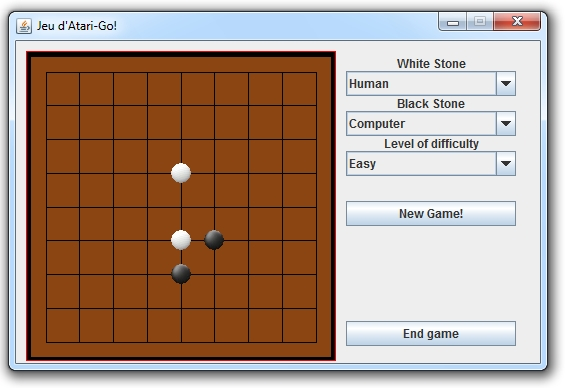
\includegraphics[width=0.75\textwidth] {img/Game.jpg}
			\end{center}


		\section{Stop the computer work}
		The user can stop whenever he wants the computer's next move deciding phase. This is helpfull to prevent long decisions (especially when the chosen level of difficulty is \empha{Hard}). For this operation, he has the \empha{End game} button. This will stop the computing and end the game on the current statement.
			\\
			\begin{center}
				
\includegraphics[width=0.30\textwidth] {img/EndGame.jpg}
			\end{center}

		\section{End of the game and display of the looser stones}
		In case there is a victory of one of the two players, a popup-window will dynamically show up, announcing the winner. This represents the end of the game. The stone or group of stones caught are framed.
			\\
			\begin{center}
				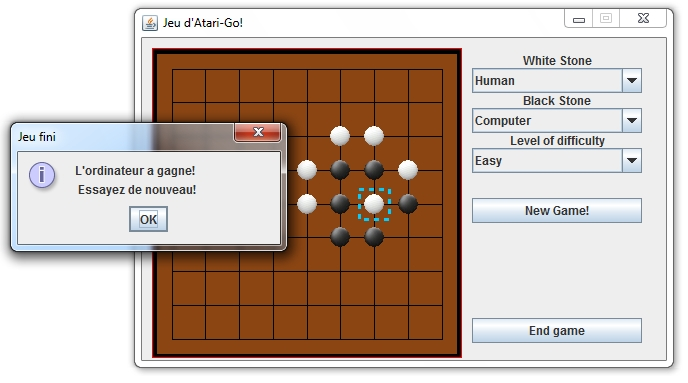
\includegraphics[width=0.75\textwidth] {img/End.jpg}
			\end{center}




	\chapter*{Developper Documentation}
		\section{Heuristic and technics}
		The chosen data structure is the \empha{Adjacency list}. A \empha{Breadth First Search} covering of the \empha{Min-Max} tree is used. A queue structure will contain bit by bit the scanned nodes. Here are the heuristics and technics used, in order to have the best complexity for the \empha{Atari-Go} game.

			\subsection{Min-Max}
			The \empha{Min-Max} algorithm works on the rule that, at each move, the computer and the human opponent will choose the best possible move. We develop a tree where for each depth we alternate the computer's move and the human opponent's move.\\
The root always represents the actual game: at the opponent level, the algorithm raises one level up-high the node having the smallest value and at the computer's level, it raises the biggest value. The operations are accomplished with a bottom-up approach. This means that it starts from the leaves and raises up the value(smallest of biggest, according to the depth) to the root.

			\subsection{Alpha-Beta}
			This technique allows to significantly reduce the number of evaluated nodes by the \empha{Min-Max} algorithm. The \empha{Alpha-Beta} prunning simply avoids the evaluations of research tree's nodes for which we are sure that the value will not be accepted from a node of a smallest deapth, which has already been evaluated. Then, it is very interesting to use this algorithm in the development of the tree of our Atari-Go game which takes part very well in it.

			\subsection{A$^*$}
			The research \empha{$A^*$} algorithm is a best-first graph search algorithm between a root node and the leaves. It is often used in \empha{Artificial Inteligence} due to its rapidity of execution. It has been created such that only some of the best solutions are treated in first place.
\\
We use this algorithm in order to do a prunning of the sons to develop for each parent node. Only a number at most equal to the tree's arity of the best sons will be developed. Moreover, to chose the best sons, it will be necessary to evaluate all the possible sons of the parent node; in an incremental way, beginning to the root state of the game.

			\subsection{Complexity}
			Thanks to the use of these different algorithms, we obtain a complexity in worst case of the approach, according to the chosen arity or the chosen depth:
			\begin{center}
				$	O(depth, exponential) = (exponential ^{(depth - 2)} ) * 81^2	$
			\end{center}
			where we consider the root at depth 1.




			\subsection{Evaluation Function}
The evaluation function totally depends on the current state of the game. Then, the state of the Goban at one instant will determinate the value of the evaluation function.
\\
This function returns an evaluation of the current game. It will be positive if the state is desirable for the computer, or negative in the contrary case. Moreover, the value is a even bigger positive number if the computer wins and a small negative number is the human opponent wins. The situation of the victory could be met in the development of the tree. In addition, we know that we dont have to develop a node \empha{victory node}, because it is final. We did not implement this \textsl{shortcut} yet, but we imagine the possibility to add it in the future code, which would avoid some calculations in the  \empha{Min-Max}  and \empha{Alpha-Beta} algorithms.
\\
Each case taken by a stone in the goban corresponds in our evaluation to an addition of a number of points; either positive or negative. We have a positive number if the number of freedoms is superior to 3 and that the stone of is one of the computers ones, or if the number of freedoms is inferior or equal to 3 and that the stone is one of the human opponent's one. All the other cases correpond to negative additions, of same modulo than the additions in the computer's favorable cases. Therefore, the computer's strategy is balanced, half oriented on defense and half on attack. When a stone is the computer's one and that the number of liberties is superior to 3, we obtain twice the number of freedoms as prize. If this is an opponent's one, with the same number of freedoms, we will get the same value, but in modulo, because it would be a negative sign. When the stone is one of the computer's one, and the it has less than 4 liberties, the result of the points for the respective intersection is like this:
			\\
			\begin{itemize}
				\item -10 points for 3 freedoms; 
				\item -10 points for 3 freedoms;
				\item -50 points for 2 freedoms;
				\item -100 points for 1 freedoms;
				\item -1000 points for 0 freedoms, then the human opponent has won.
			\end{itemize}

Obviously, as previously noticed, if the number of freedoms are same, but for an intersection containing a stone of a human player. The result will be the same in modulo, but the sign stays positive.


		\section{Oganization of the project}

			\subsection{General}
				The project has been made, in the begining, to be supported by \empha{Subversion} system. At the root of the project, you will meet the SVN folders. Then, in the \empha{Trunk} folder there is a \empha{Maven} architecture. All folders have been integrated into the \empha{Eclipse} project.
\\
				This organization allows to easily share the project to anyone who wants to contribute to its development, via the \empha{SVN} system, but also, it can allow people to compile, and generate all tools that Maven gives through its engine. And finaly, the \empha{Eclipse} project has been chosen, because Eclipse is the most used \empha{Integrated Development Environment for Java}.
\\
				Here is the tree architecture of the whole project:
\\
				\begin{center}
					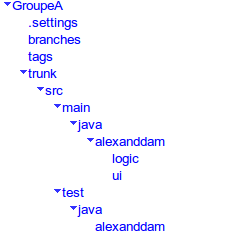
\includegraphics[width=0.50\textwidth] {img/tree.png}
				\end{center}


			\subsection{Eclipse project}
					The first folders of the architecture are then the \empha{Eclipse} project. You can find there, the normal \empha{.settings} folder, the  \empha{.classpath} and  \empha{.project} files at the very root of the whole project architecture.


			\subsection{SVN project}
				The project is also available on the web, for everyone who wants to contribute:  \href{http://code.google.com/p/alma-go/}{http://code.google.com/p/alma-go/}

					\begin{itemize}
						\item \textbf{trunk}\\
							This folder will usually contain the most recent version of the data, the whole project is here.
						\item \textbf{branches}
							The branches folder will contain any code that was branched from the main trunk. We actually don't have any branch of the project. Thus, the folder is empty.
						\item \textbf{tags}
							Whenever a new release is made, a new tag will be created in this folder. A tag is basically a snapshot of the repository at a certain point in time. We have here the nightsnapshot.
					\end{itemize}

			\subsection{Maven project}
				\empha{Maven} is a software tool for Java project management and build automation. We respected the folder architecture plan of Maven. The whole code is in the \empha{src} folder. Here are the two \empha{main} folders: the main code of the application and the \empha{test} folder, which regroups the JUnit test classes.
\\
				The main tools installed in the \empha{pom.xml}, which help the developper are:

					\begin{itemize}
						\item \textbf{Site}\\
							Executing: \\ \empha{mvn site}\\ you will generate the project website, the PMD checkstyle report and the Javadoc. This will create the \empha{target} folder with the website as content.
						\item \textbf{Javadoc}\\
							You also can generate the javadoc in standalone, just executing:\\ \empha{mvn javadoc:javadoc}\\ This will also generate the javadoc website, in the  \empha{target folder}.

						\item \textbf{Package}\\
							We configured the \empha{package} plugin of Maven, in order to generate an executable jar of our project :  \empha{almago-1.0-SNAPSHOT.jar} . Execute:\\ \empha{mvn package}.

					\end{itemize}










		\section{Annalyse}
		The use of the Java programming language has been imposed for our project. Moreover, the \empha{Oriented Object Programming} appeared to us obvious, for the clarity of the code and a better team division.
\\
Here is the UML diagramm of the architecture of the application:
			\\
			\begin{center}
				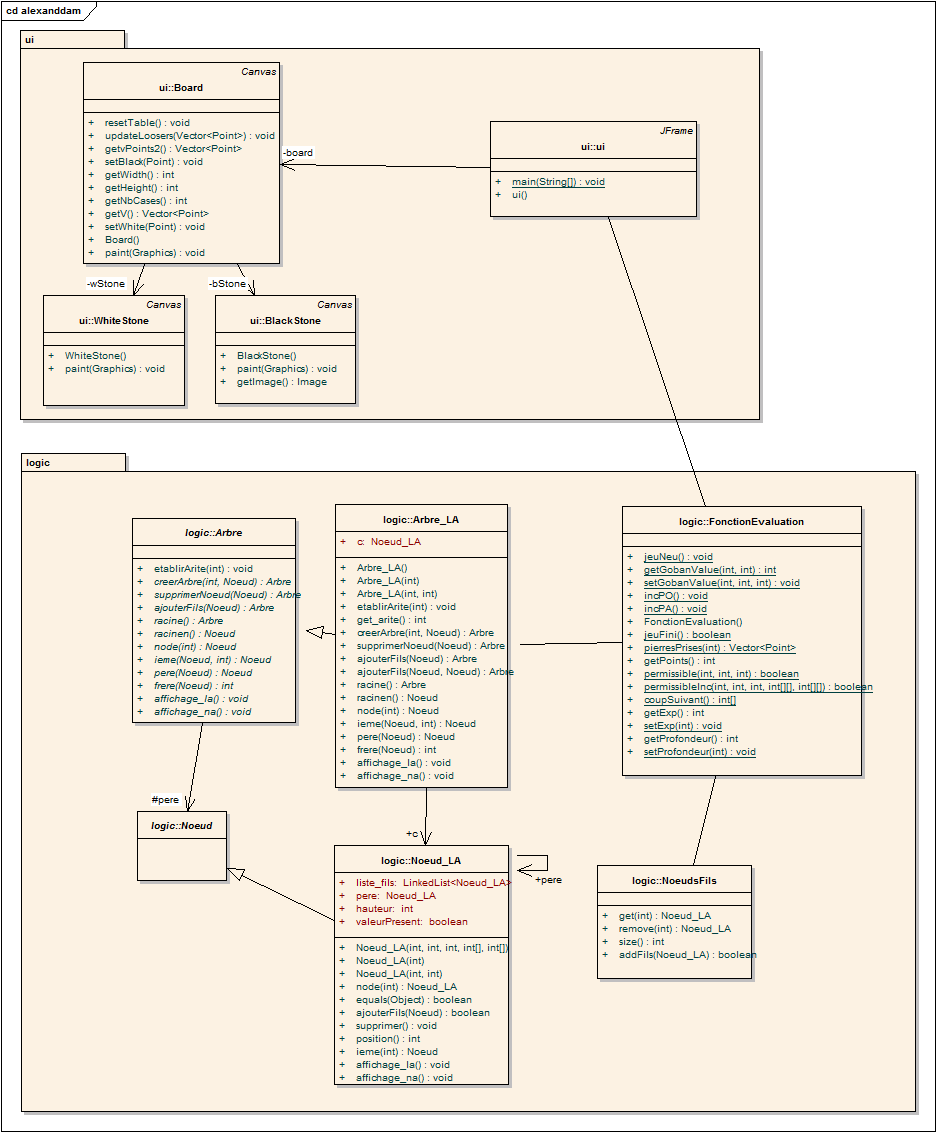
\includegraphics[width=\textwidth] {img/uml.png}
			\end{center}

		\section{Implementation}
		This is the first section of the second chapter.

			\subsection{Package \empha{ui}}
			\begin{itemize}

				\item \textbf{UI} Class\\
This class is the main class of the \empha{Java} program \empha{Atari-Go game}, containing the Graphical User Interface and linking it to the \empha{Arficial Inteligence} engine.
The level of difficulty of the computer is proposed in different value pairs of (depth, exponentional):
					\begin{itemize}
						\item (7.30) for \empha{Hard}
						\item (5.20) for \empha{Medium}
						\item (5.10) for \empha{Easy}
						\item (3.80) for \empha{Very Easy}
					\end{itemize}
In order to notify to the user that the system is working, developping the \empha{Min-Max} tree which can become long, the cursor becomes a \empha{Wait\_Cursor} and turns again to the \empha{Default} once the move is played by the computer.

				\item \textbf{Board} Class\\
This is a \empha{Java Canvas}, which draws the Goban, the "played" stones and frame the loosing stones at the end of the game.

				\item \textbf{WhiteStone} Class\\
This class represents the white stones of the \empha{Atari-Go} game, and extends the \empha{Java Canvas}.

				\item \textbf{BlackStone} Class\\
This class represents the black stones and also extends the \empha{Java Canvas}.

			\end{itemize}

			\subsection{Package \empha{logic}}
This package represents the main part of the software: the \empha{Artificial Inteligence} engine.
			\begin{itemize}
				\item \textbf{FonctionEvaluation} Class\\
The \empha{FonctionEvaluation} Class is the main class of the logical part of the software. This gives the development of the \empha{Min-Max} tree, in order to give the next move of the computer, from any state of the game (except ended game, obviously).
\\
In this class are listed the previouly named technics and heuristics. The main function of those are then:
			\begin{itemize}
				\item Calculate the stones freedoms.
				\item Calculate the permission of the current move (non suicide, already played stone ...).
				\item Calculate the evaluation of the actual game or the one represented by the a node in the Min-Max tree.
				\item Check the victory of a player.
				\item Calculate the taken stones.
				\item Develop the Alph-Beta tree, using the incremental evaluation function.
			
			\end{itemize}

				\item \textbf{NoeudsFils} Class \\
This class gives the management and the use of the \empha{$A^*$} algorithm imbricated in the \empha{Min-Max}.
\\
The class acutally manages a specific data structure of type list: \empha{ArrayList}. This list containts the sons of a parent node in an ordered way. The order is realised according to the evaluation function, then according to the value which is contained in the Node structure. Bit by bit, we try to add new nodes in the list, scanning to see where is the location of the new node. This way, the order is kept. We try, because the size of the list is given by an exponential value or otherwise called: \empha{Arity} of the tree. The arity depends of the level of difficulty, chosen by the user. In the case of node \empha{max}, the list is ordered in a increasing order and in the case of a \empha{min} node, it is in a decreasing order. Therefore, the best nodes are always at the end of the structure. Moreover, a simple comparison is enough to not have to scan the whole list and see whether our element is already in it or not.

				\item \textbf{Arbre\_LA} Class \\
Implementation of the \emph{Arbre} abstract class, this class creates the tree as \empha{Adjacency list}. The adjacency list is the way to create the \empha{Min-Max} tree, knowing that the number of sons of each node is not constant. More, the use of the \empha{Modular Array} is not desirable.

				\item \textbf{Noeud\_LA} Class\\
The class \empha{Noeud\_LA} is the concrete implementation of the abstract class \emph{Noeud}. This class is then the useful class in the tree data structure. It contains the basic management of the nodes in the tree  of the previous \empha{Arbre\_LA} class.

				\item \textbf{Arbre} Class\\
					This abstract class list the functions needed for the management of a tree data structure which is useful for the use of the \emph{Min-Max} algorithm.

				\item \textbf{Noeud} Class\\
					The class \empha{Noeud} is an abstract class, used for the tree data structure. It contains the vectors of coordinates of the computer moves, of the human player moves and the values issued from the evaluation function for the actual game which is described by the respective nodes.

			\end{itemize}

\end{document} 




















